\section{Aufbau}
\begin{figure}
	\centering
	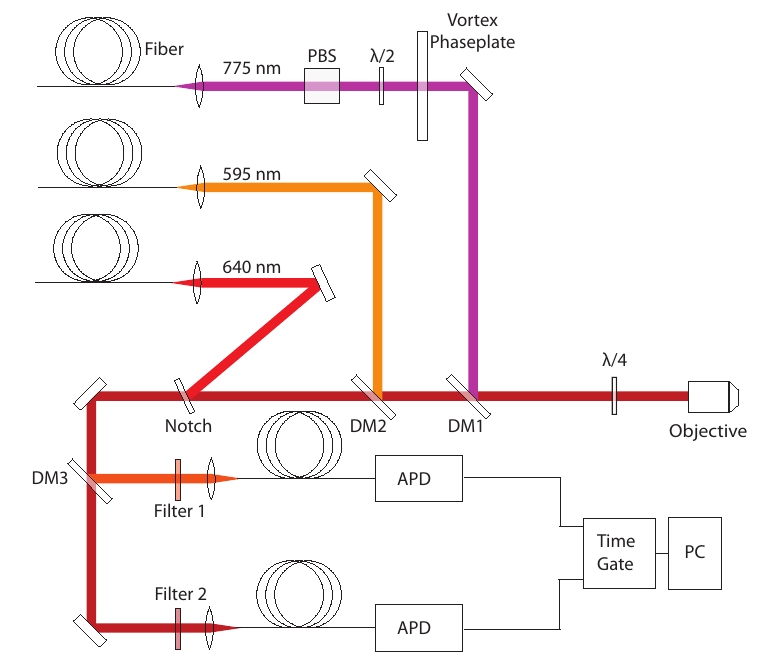
\includegraphics[width=0.75\textwidth]{plots/aufbau.png}
	\caption{Skizze des Aufbaus. Der Laser der Wellenlänge 595~nm und der Detektionspfad dieses Strahls kommen in diesem Versuch nicht zum Einsatz.}
\end{figure}
Zur STED-Mikroskopie in diesem Versuch wird ein 640~nm Laser als Anregungslaser und ein 775~nm Laser als STED-Laser verwendet.
Beide Laser sind gepulst und werden mithilfe von polarisationserhaltenden Fasern in den Aufbau eingebracht und mit Linsen kollimiert.
\\
Zur Erzeugung der Ringform des STED-Lasers wird eine Polymer-Phasenplatte und eine $\lambda/4$-Platte verwendet.
Dafür muss der STED-Laser linear polarisiert sein, was durch einen polarisierenden Strahlteiler erreicht wird.
\\
Nachdem die Strahlen überlagert wurden werden sie in das Objektiv geleitet.
Bei dem Objektiv handelt es sich um ein \emph{Leica HCX PL APO 100X/1.40-0.70 OIL CS} mit einer numerischen Apertur von 1.4. 
Das Immersionsöl besitzt einen Brechungsindex von 1.52.
\\
Das von der Probe emittierte Fluoreszenzlicht passiert das Objektiv und die Einkoppelspiegel und wird an einen Photomultiplier (PMT) bzw. eine Avalanchephotodiode (APD) geleitet, die die Intensität über die Zahl der einfallenden Photonen misst.
